\chapter{Capteurs}
\label{chap:sensors}

\section{Classification des capteurs}
\subsection{Introduction}
Les capteurs peuvent être classés selon différents critères, à savoir :
\begin{itemize}
    \item Principe de fonctionnement passif ou actif
    \item Type de mesure absolue ou relative
    \item Les types de matériaux utilisés
    \item Les principes de mesures
    \item Les stimuli utilisés
    \item Les champs d'application
\end{itemize}

Dans ce chapitre nous listerons les critères de classement et nous présenterons quelques exemples de capteurs au travers de leur fiche de spécification.
Et n'oubliez pas le système mksA (mètre, kilogramme, seconde, Ampère, ...) ou système international d'unités de mesure vu précédemment. Le tableau \ref{fig:Systeme_international_d_unites_SI} donne un bref rappel des 7 unités physiques de base indépendantes.

\begin{figure}[h!]
    \centering
    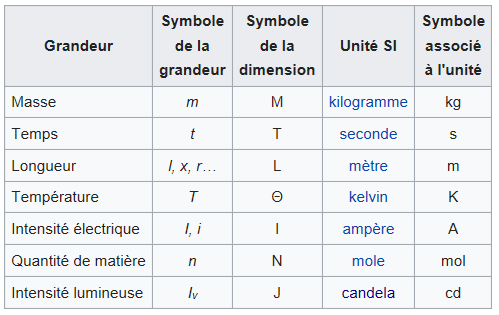
\includegraphics[height=6cm]{assets/figures/4_1_2_Systeme_international_d_unites_SI.PNG}
    \caption{Système international d'unités SI: les 7 unités physiques de base.}
    \label{fig:Systeme_international_d_unites_SI}
\end{figure}

\section{Choix d'un capteur}

Le choix du capteur approprié dépend du cahier des charges. Les conditions imposées sur la valeur à mesurer imposent des caractéristiques métrologiques sur le capteur.
\begin {center}
\begin{tabular}{|p{6cm}|p{6cm}|}\hline
    \textbf{MESURANDE}                          & \textbf{CAPTEUR}                                  \\
    Conditions imposées                         & Caractéristiques métrologiques                    \\\hline\hline
    Plage de variation                          & Étendue de mesure                                 \\\hline
    Variation minimale à mesurer                & Résolution                                        \\\hline
    Spectre de fréquence ou vitesse de rotation & Bande passante                                    \\\hline
    Précision de mesure                         & Erreur de linéarité, Erreur d'hystérésis          \\\hline
    Plage de température de fonctionnement      & Dérive thermique du zéro, Tenue en température    \\\hline
    Localisation                                & Encombrement                                      \\\hline
    Composition de l'atmosphère                 & Inertie chimique, Protection                      \\\hline
    Parasites                                   & Blindage, Isolement ou non par rapport à la masse \\\hline
\end{tabular}
\end{center}
Source : www.geea.org

Ces conditions concernent autant le paramètre à mesurer (par exemple la pression) que l'environnement de mesure. Elles doivent être traduites en caractéristiques métrologiques du capteur. Ces caractéristiques sont à comparer à celles se trouvant dans les fiches techniques du capteur.

Le choix du bon capteur consiste à trouver des caractéristiques qui englobent les conditions imposées sur la mesurande.

\subsection{Principaux termes utilisés pour spécifier les capteurs}

Un grand nombre de paramètres spécifient un capteur. Ces paramètres sont identifiés par les termes du tableau ci-dessous.
\begin {center}
\begin{tabular}{|p{2.2cm}|p{2.8cm}|p{6.8cm}|p{2.4cm}|}
    \hline
    \textbf{Français}            & \textbf{Anglais}         & \textbf{Définition}                                                                                                     & \textbf{exemple}                \\
    \hline
    \hline
    Sensibilité                  & Sensitivity              & output variation / input variation                                                                                      & mV/g, mA/oC                     \\
    \hline
    Stabilité                    & Stability                & Coefficient de variation selon une grandeur d'influence                                                                 & stabilité en température        \\
    \hline
    Précision                    & Accuracy                 & Somme de toutes les perturbations qui influencent la sortie du capteur                                                  &                                 \\
    \hline
    Étendue de mesure            & Span, range              & Valeur max mesurable - valeur min mesurable                                                                             &                                 \\
    \hline
    Résolution                   & Resolution               & Plus petite variation du mesurande mesurable par le capteur                                                             &                                 \\
    \hline
    Sélectivité                  & Selectivity              & S'applique à des capteurs biochimiques, sensibles à une molécule plus particulièrement par rapport à une autre molécule &                                 \\
    \hline
    Temps de réponse             & Response time            & Temps de propagation entre l'entrée et la sortie du capteur                                                             &                                 \\
    \hline
    Conditions environnementales & Environmental conditions & Décrit les plages de variation admissible pour les paramètres extérieurs                                                & humidité, température, pression \\
    \hline
    Facteur de surcharge         & Overload characteristics & Capacité à supporter un dépassement de la plage de mesure du mesurande                                                  &                                 \\
    \hline
    Linearité                    & Linearity                &                                                                                                                         &                                 \\
    \hline
    Hystérèse                    & Hysteresis               &                                                                                                                         &                                 \\
    \hline
    Zone morte                   & Dead band                & Plage de valeur du mesurande pour laquelle la sensibilité du capteur est nulle ou mauvaise                              &                                 \\
    \hline
    Durée de vie                 & Operating life           & Durée pendant laquelle les caractéristiques du capteur sont observées                                                   & mtbf = mean time before failure \\
    \hline
    Taille                       & Size                     &                                                                                                                         &                                 \\
    \hline
    Poids                        & Weight                   &                                                                                                                         &                                 \\
    \hline
    Prix                         & Price                    &                                                                                                                         &                                 \\
    \hline
\end{tabular}
\end{center}

Il existe des capteurs actifs et passifs :
\begin{center}
    \fbox{
        \begin{minipage}{0.95\textwidth}
            \textbf{\textit{Déf}. Capteur actif :}
            n'a pas besoin d'énergie additionnelle: génère un signal électrique en réponse à un stimulus externe. Exemples: thermocouples, capteur pyroélectrique, capteur piézoélectrique. \\

            \textbf{\textit{Déf}. Capteur passif :}
            il s'agit généralement d'impédances. Les capteurs passifs nécessitent une énergie externe pour fonctionner, appelé signal d'excitation. Ce signal est modulé par le capteur pour produire le signal de sortie. Ces capteurs sont parfois appelés paramétriques, car leur signal de sortie change en fonction de ce signal d'excitation.
        \end{minipage}
    }
\end{center}

Les capteurs peuvent aussi être absolus ou relatifs, avec comme définitions :
\begin{center}
    \fbox{
        \begin{minipage}{0.95\textwidth}
            \textbf{\textit{Déf}. Capteur absolu :}
            détecte  un mesurande et produit une sortie en relation directe avec une échelle physique absolue indépendante des conditions de mesure. Exemple: résistance à coefficient de température positif, sa résistance dépend de la température absolue. \\

            \textbf{\textit{Déf}. Capteur relatif :}
            la sortie d'un capteur relatif dépend du contexte, d'une autre grandeur. Par exemple le signal de sortie d'un thermocouple ne peut être associé à une température absolue sans référencer l'une de ses extrémités à une température connue. Autre exemple, un capteur de pression peut être absolu lorsque son signal de sortie dépend de la différence entre la pression d'entrée et une pression de référence interne, ou relatif lorsqu'il est nécessaire d'appliquer une pression de référence de manière externe.
        \end{minipage}
    }
\end{center}

\section{Matériaux utilisés dans la réalisation de capteurs}

Différents matériaux sont utilisés pour la réalisation de capteurs.

\begin {center}
\begin{tabular}{|p{4.2cm}|p{9.5cm}|}
    \hline
    Organique              & Matière fabriquée par les êtres vivants                                                                                                                                                                                                                                                                                                 \\
    \hline
    Inorganique            & Matière qui ne possède pas les caractéristiques nécessaires à la vie                                                                                                                                                                                                                                                                    \\
    \hline
    Conducteur             & Corps capable de transmettre de l'électricité                                                                                                                                                                                                                                                                                           \\
    \hline
    Isolant                & Matériau qui isole de l'électricité                                                                                                                                                                                                                                                                                                     \\
    \hline
    Semi-conducteur        & matériau qui a les caractéristiques électriques d'un isolant, mais pour lequel la probabilité qu'un électron puisse contribuer à un courant électrique, quoique faible, est suffisamment importante. En d'autres termes, la conductivité électrique d'un semi-conducteur est intermédiaire entre celle des métaux et celle des isolants \\
    \hline
    Liquide, gaz ou plasma & Etats de la matière                                                                                                                                                                                                                                                                                                                     \\
    \hline
    Substance biologique   & Matériau extrait du monde vivant                                                                                                                                                                                                                                                                                                        \\
    \hline
\end{tabular}
\end{center}

\section{Principes de conversion}

Le mesurande doit être converti dans une grandeur exploitable. Cela nécessite un principe physique reliant cette grandeur au mesurande. Voici une liste non exhaustive de principes physiques se retrouvant dans les capteurs :

\begin {center}
\begin{tabular}{|p{4.2cm}|p{9.5cm}|}
    \hline
    Physiques   & Piézoélectricité               \\
    \hline
                & Thermoélectrique               \\
    \hline
                & Photoélectrique                \\
    \hline
                & Photomagnétique                \\
    \hline
                & Magnétoélectrique              \\
    \hline
                & Électromagnétique              \\
    \hline
                & Thermoélastique                \\
    \hline
                & Electroélastique               \\
    \hline
                & Thermomagnétique               \\
    \hline
                & Thermo-optique                 \\
    \hline
                & Photoélastique                 \\
    \hline
                & ...                            \\
    \hline
    Chimiques   & Transformation chimique        \\
    \hline
                & Transformation physique        \\
    \hline
                & Processus électrochimique      \\
    \hline
                & Spectroscopie                  \\
    \hline
                & ...                            \\
    \hline
    Biologiques & Transformation biochimique     \\
    \hline
                & Transformation physique        \\
    \hline
                & Effet sur un organisme de test \\
    \hline
                & Spectroscopie                  \\
    \hline
                & ...                            \\
    \hline
\end{tabular}
\end{center}

\section{Le mesurande}
Le mesurande est un terme défini comme étant la grandeur que l'on veut mesurer. La définition du mesurande est un préalable essentiel dans tout processus de mesure. Une liste non exhaustive de mesurandes :

%\begin{multicols}{2}
\begin {center}
\begin{tabular}{|p{3cm}|p{7cm}|}
    \hline
    Onde & acoustique	amplitude \\
    \hline
         & phase               \\
    \hline
         & polarisation        \\
    \hline
         & spectre             \\
    \hline
         & vélocité            \\
    \hline
\end{tabular}
\begin{tabular}{|p{3cm}|p{7cm}|}
    Biologique & type de biomasse \\
    \hline
               & concentration    \\
    \hline
               & états            \\
    \hline
\end{tabular}
\begin{tabular}{|p{3cm}|p{7cm}|}
    Chimique & type de composants \\
    \hline
             & concentration      \\
    \hline
             & états              \\
    \hline
\end{tabular}
\begin{tabular}{|p{3cm}|p{7cm}|}
    Électrique & charge, courant    \\
    \hline
               & potentiel, tension \\
    \hline
               & champ électrique   \\
    \hline
               & conductivité       \\
    \hline
               & permittivité       \\
    \hline
\end{tabular}
\begin{tabular}{|p{3cm}|p{7cm}|}
    Magnétique & amplitude    \\
    \hline
               & phase        \\
    \hline
               & polarisation \\
    \hline
               & spectre      \\
    \hline
               & flux         \\
    \hline
               & perméabilité \\
    \hline
\end{tabular}
\begin{tabular}{|p{3cm}|p{7cm}|}
    Onde optique & amplitude            \\
    \hline
                 & phase                \\
    \hline
                 & polarisation         \\
    \hline
                 & spectre              \\
    \hline
                 & vélocité             \\
    \hline
                 & indice de réfraction \\
    \hline
                 & émissivité           \\
    \hline
                 & réflectivité         \\
    \hline
                 & absorption           \\
    \hline
\end{tabular}
\begin{tabular}{|p{3cm}|p{7cm}|}
    Mécanique & position linéaire       \\
    \hline
              & position angulaire      \\
    \hline
              & force                   \\
    \hline
              & tension, pression       \\
    \hline
              & contrainte              \\
    \hline
              & masse, densité          \\
    \hline
              & moment, couple          \\
    \hline
              & vitesse                 \\
    \hline
              & forme, état de surface  \\
    \hline
              & orientation             \\
    \hline
              & cristalinité, structure \\
    \hline
\end{tabular}
\begin{tabular}{|p{3cm}|p{7cm}|}
    Radiation & type      \\
    \hline
              & énergie   \\
    \hline
              & intensité \\
    \hline
\end{tabular}
\begin{tabular}{|p{3cm}|p{7cm}|}
    Thermique & température            \\
    \hline
              & flux thermique         \\
    \hline
              & chaleur spécifique     \\
    \hline
              & conductivité thermique \\
    \hline
\end{tabular}
\end{center}
~\\
%\end{multicols}

Le \textbf{mesurage}, c'est l'ensemble des opérations pour déterminer la valeur du mesurande, dont le résultat est la \textbf{mesure}.

Parfois, la valeur que l'on peut mesurer n'est pas la valeur que l'on veut mesurer. La grandeur mesurée n'est alors pas équivalente au mesurande. Par exemple, si les conditions de mesure ne sont pas adéquates, il est alors nécessaire d'effectuer une correction de la valeur mesurée. Exemple : en voulant mesurer la longueur d'une pièce mécanique à $20 \degree C$, alors que sa température réelle est de $80 \degree C$, il est nécessaire d'effectuer une correction due à la dilatation (entre $20 \degree C$ et $80 \degree C$).

\section{Capteur réel}
L'écart entre la valeur vraie et la valeur mesurée s'appelle l'erreur de mesure. Un capteur réel souffre de plusieurs erreurs caractéristiques (source : www.geea.org) :

\begin{figure}[h!]
    \centering
    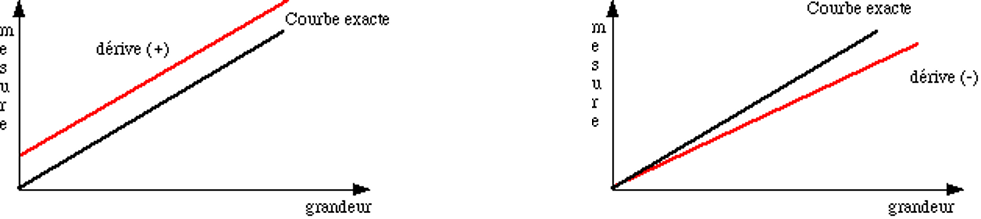
\includegraphics[width=\textwidth]{assets/figures/4_1_8_Erreurs_de_decalage_et_de_gain.PNG}
    \caption{Erreurs de décalage et de gain}
    \label{fig:Erreurs_de_decalage_et_de_gain}
\end{figure}

\begin{figure}[h!]
    \centering
    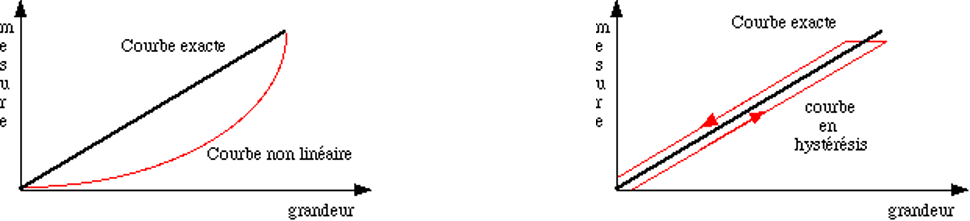
\includegraphics[width=\textwidth]{assets/figures/4_1_8_Erreurs_de_linearite_et_d_hysterese.PNG}
    \caption{Erreurs de linéarité et d'hystérèse}
    \label{fig:Erreurs_de_linearite_et_d_hysterese}
    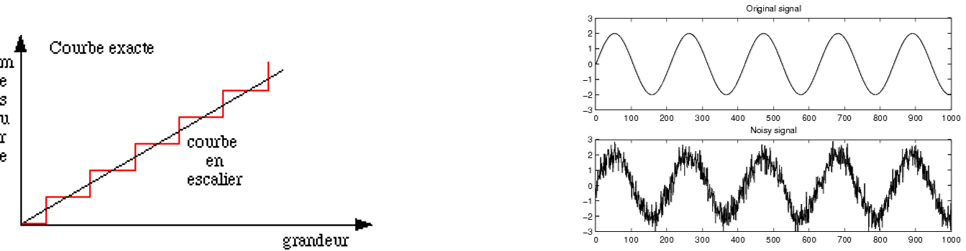
\includegraphics[width=\textwidth]{assets/figures/4_1_8_Erreurs_de_mobilite_et_bruit.PNG}
    \caption{Erreurs de mobilité et bruit}
    \label{fig:Erreurs_de_mobilite_et_bruit}
\end{figure}
Il faut en particulier différencier les erreurs systématiques et les erreurs aléatoires. L'erreur systématique est un décalage entre la valeur vraie et la valeur mesurée. L'erreur aléatoire peut se situer de part et d'autre de la valeur vraie.
\begin{figure}[h!]
    \centering
    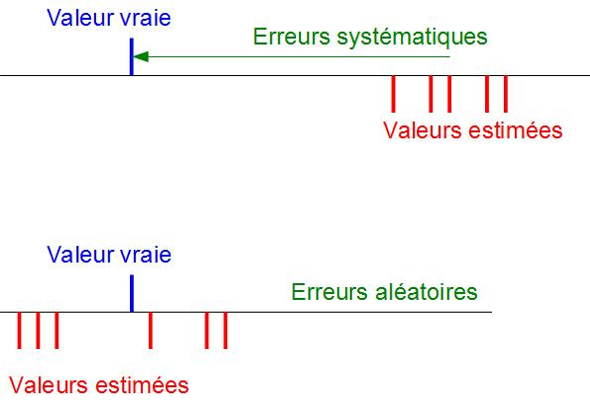
\includegraphics[height=6cm]{assets/figures/4_1_8_Erreurs_systematiques_et_aleatoires.PNG}
    \caption{Erreurs systématiques et aléatoires}
    \label{fig:Erreurs_systematiques_et_aleatoires}
\end{figure}
Les notions de justesse et de fidélité (ou répétabilité) sont associées à ces erreurs systématiques et aléatoires.

\section{Exemples de capteurs}

\subsection{Grandeurs électriques}

\subsubsection{Capteur de courant inductif}

Différent principaux permettent la mesure du courant électrique. Le transformateur de courant est une technique inductive basé sur un transformateur ayant au primaire une ou plusieurs spires avec le fil où la mesure de courant est effectuée. Au secondaire se trouve un ampèremètre. Le ratio entre le courant du secondaire et du primaire est proportionnel au rapport du nombre de spires entre le primaire et le secondaire.
\begin{figure}[h!]
    \centering
    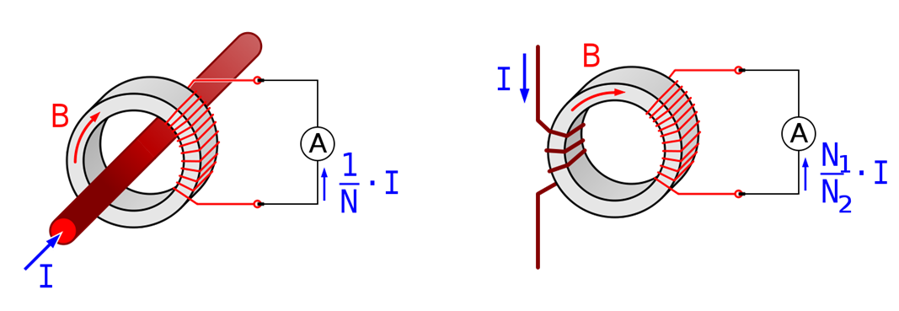
\includegraphics[height=5cm]{assets/figures/4_2_1_1_Capteur_de_courant_inductif.PNG}
    \caption{Capteur de courant inductif (Source : Wikipedia).}
    \label{fig:Capteur_de_courant_inductif}
\end{figure}

\subsubsection{Bobine de Rogowski}

La bobine de Rogowski est un cas particulier de mesure inductive sans entrefer. Il s'agit d'un solénoïde particulier placé autour du conducteur. La tension induite est peu/pas dépendante de la position du conducteur dans la boucle.

\begin{figure}[h!]
    \centering
    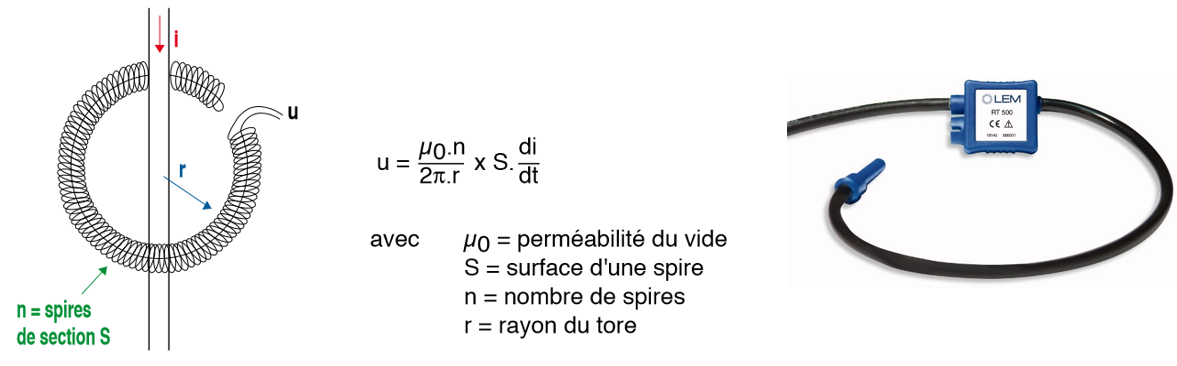
\includegraphics[width=15cm]{assets/figures/4_2_1_2_Bobine_de_Rogowski.PNG}
    \caption{Bobine de Rogowski (Sources : Chauvin-Arnoux et LEM).}
    \label{fig:Bobine_de_Rogowski}
\end{figure}


\subsubsection{Capteur de courant par effet Hall}
D'autres principes permettent de mesurer le courant, comme par exemple un capteur à effet Hall mesurant le champ magnétique autour du conducteur. Cette solution a comme gros avantage, par rapport aux techniques inductives, de permettre la mesure des courants continus.


\begin{figure}[h!]
    \centering
    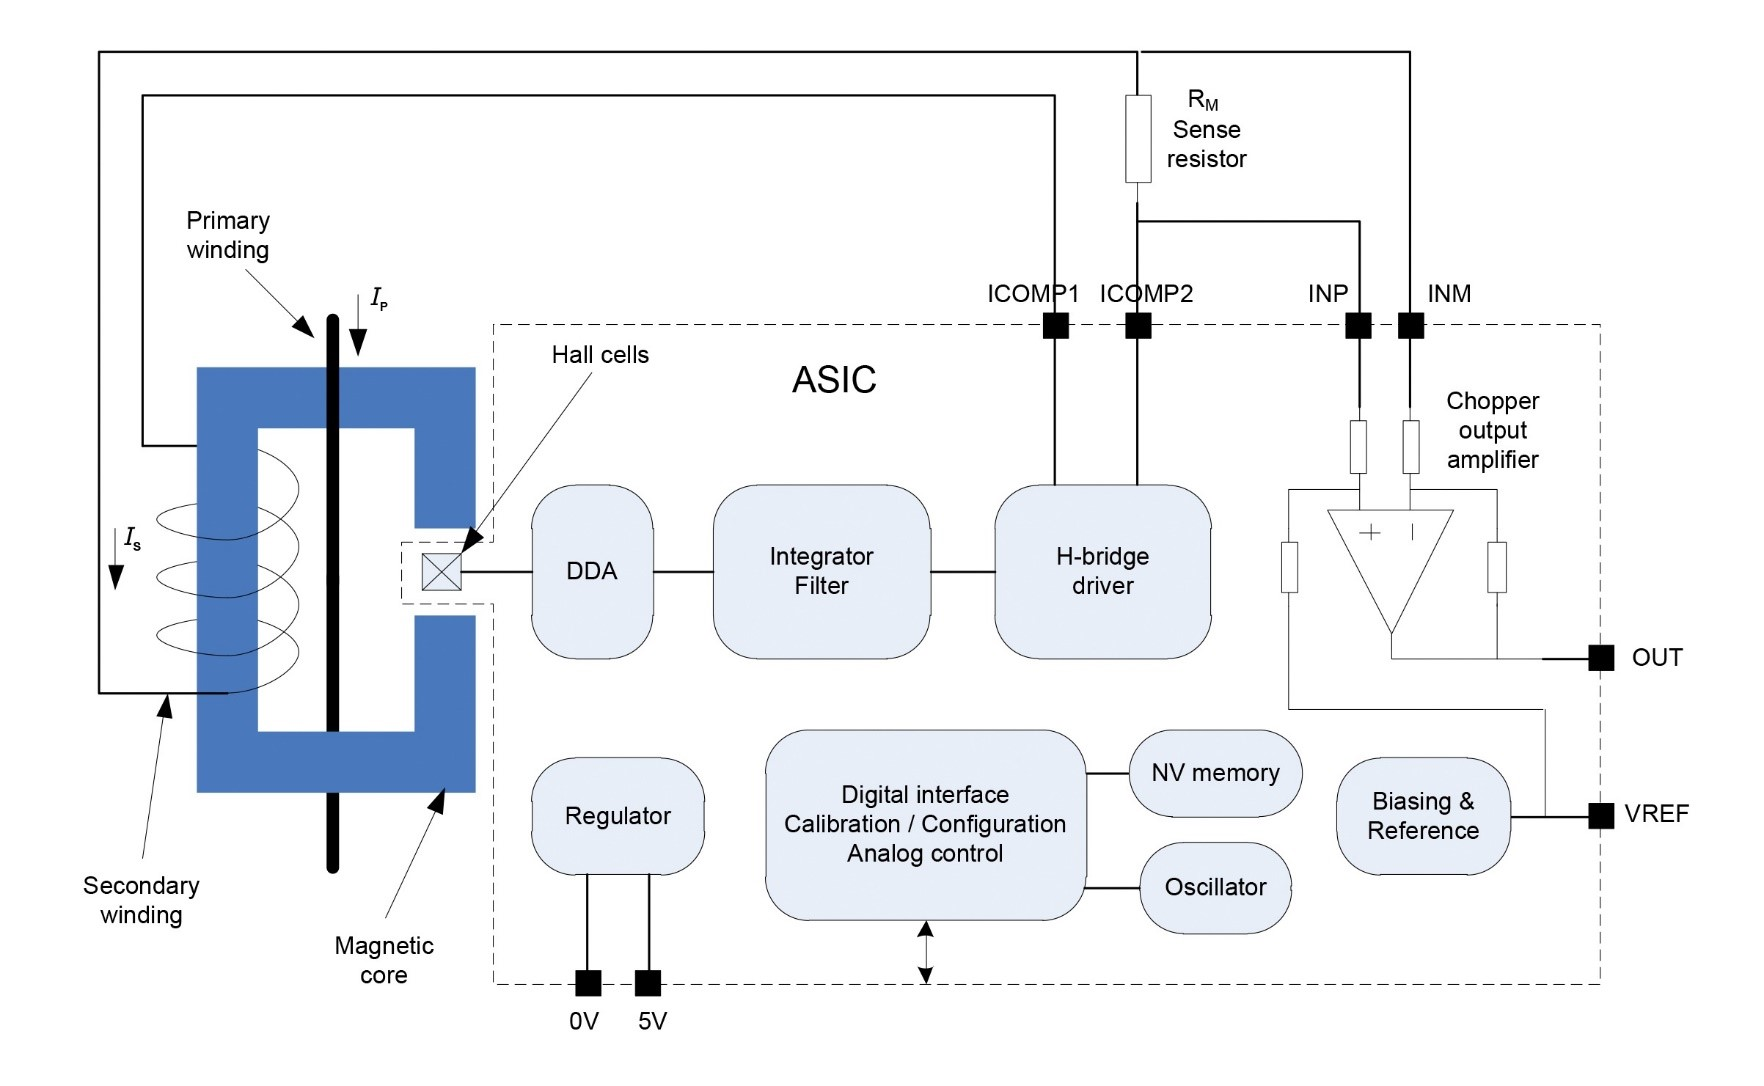
\includegraphics[width=15cm]{assets/figures/4_2_1_2_Capteur_de_courant_par_effet_Hall.jpg}
    \caption{Capteur de courant par effet Hall (Source: LEM).}
    \label{fig:Capteur_de_courant_par_effet_Hall}
\end{figure}

Ci-joint se trouve le schéma d'un capteur intelligent permettant la mesure en boucle fermée. Une contre-réaction permet de générer un champ magnétique s'opposant au champ magnétique lui-même généré par le courant à mesurer. Une structure à contre-réaction offre le grand avantage d'être sensible aux caractéristiques de la bobine plutôt qu'à la sensibilité du capteur à effet Hall.

\subsection{Température (TMP75 de Texas Instruments)}
Le TMP75 de Texas Instrument est un capteur intelligent disposant d'une interface I2C.

\begin{figure}[h!]
    \centering
    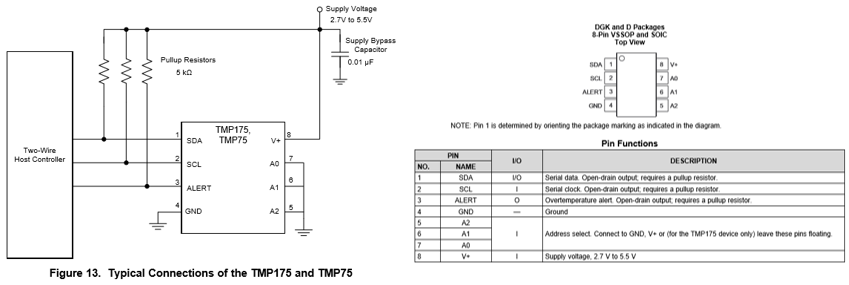
\includegraphics[width=15cm]{assets/figures/4_2_2_Temperature_TMP75.PNG}
    \caption{Mesure de température avec le circuit TMP75}
    \label{fig:Temperature_TMP75}
\end{figure}

Il se connecte aisément à un hôte, comme un microcontrôleur avec les deux signaux SDA et SCL. Une ligne supplémentaire ALERT permet en particulier de déclencher des interruptions.

Ce capteur intelligent dispose d'une cellule de mesure (Diode Temp. Sensor dans le schéma bloc ci-dessous), d'un convertisseur analogique numérique (convertisseur $ \Delta \Sigma$) et numérique-analogique.


\begin{figure}[h!]
    \centering
    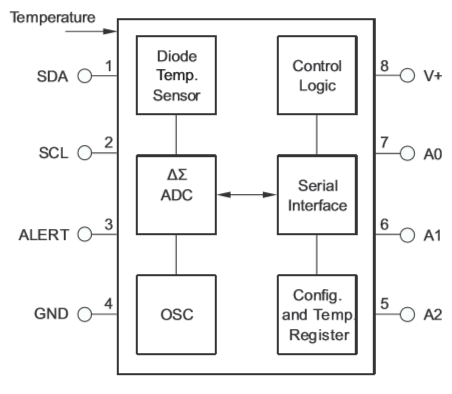
\includegraphics[height=6cm]{assets/figures/4_2_2_Temperature_TMP75_schema_bloc.PNG}
    \caption{Schéma bloc circuit TMP75}
    \label{fig:Temperature_TMP75_schema_bloc}
\end{figure}

Pour un capteur de température, la fiche technique donne un grand nombre de paramètres, comme en particulier les caractéristiques électriques ci-dessous. Chaque caractéristique peut avoir une grande importance pour une application.

\begin{figure}[h!]
    \centering
    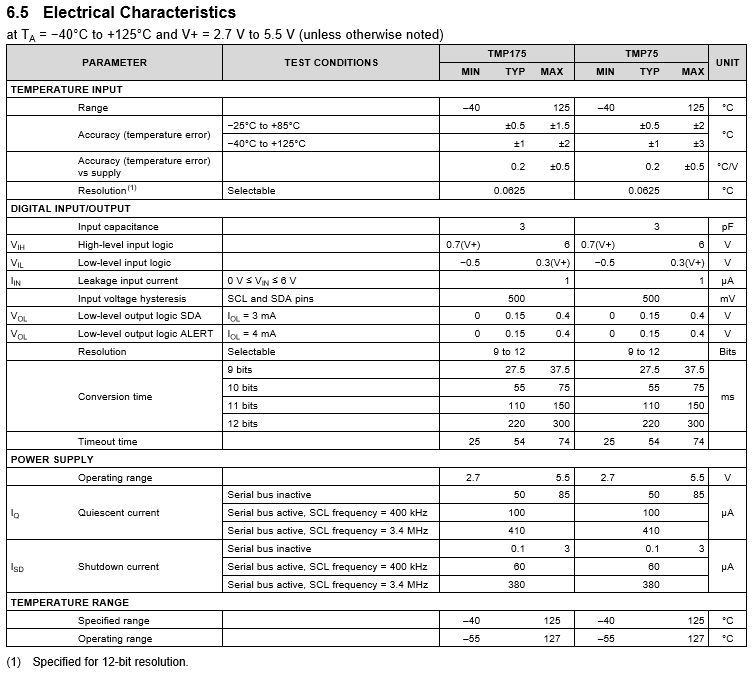
\includegraphics[width=15cm]{assets/figures/4_2_2_Temperature_TMP75_caracteristiques.PNG}
    \caption{Caractéristiques du circuit TMP75}
    \label{fig:Temperature_TMP75_caracteristiques}
\end{figure}



\subsection{Humidité (SHT3x-ARP de Sensirion)}
\begin{figure}[h!]
    \centering
    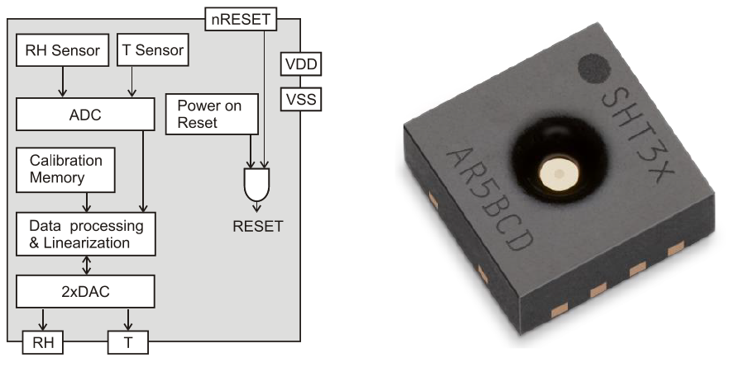
\includegraphics[width=8cm]{assets/figures/4_2_3_Humidite_SHT_3x_ARP.PNG}
    \caption{Capteur d'humidité de Sensirion, SHT3x-ARP}
    \label{fig:Humidite_SHT3x_ARP}
\end{figure}


La mesure de l'humidité avec ce capteur (Sensirion SHT3x-ARP) est une tension analogique radiométrique 10\% to 90\%. Cela veut dire que la mesure est proportionnelle à la tension d'alimentation. À noter un deuxième signal de température.


\begin{figure}[h!]
    \centering
    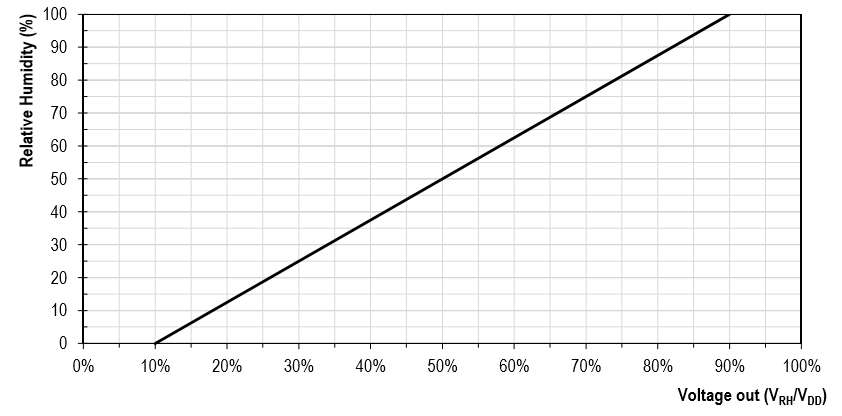
\includegraphics[width=15cm]{assets/figures/4_2_3_Humidite_SHT_3x_ARP_reponse.PNG}
    \caption{Réponse du capteur d'humidité de Sensirion, SHT3x-ARP}
    \label{fig:Humidite_SHT3x_ARP_reponse}
\end{figure}

L'incertitude de mesure se retrouve dans la fiche technique, avec une erreur typique et une erreur maximale.



\begin{figure}[h!]
    \centering
    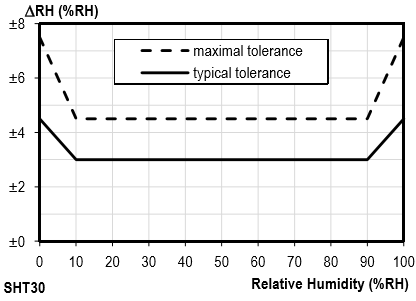
\includegraphics[width=10cm]{assets/figures/4_2_3_Humidite_SHT_3x_ARP_incertitude.PNG}
    \caption{Incertitude de mesure du capteur d'humidité de Sensirion, SHT3x-ARP}
    \label{fig:Humidite_SHT3x_ARP_incertitude}
\end{figure}

\subsection{Pression (Keller series 26 W)}
Le principe de fonctionnement de ce capteur de pression est une membrane se déformant sous l'effet de la différence de pression appliquée sur ces deux faces. Des piézorésistances (changement de résistance électrique d'un matériau dû à une contrainte mécanique) mesurent les contraintes mécaniques dans la membrane.


\begin{figure}[h!]
    \centering
    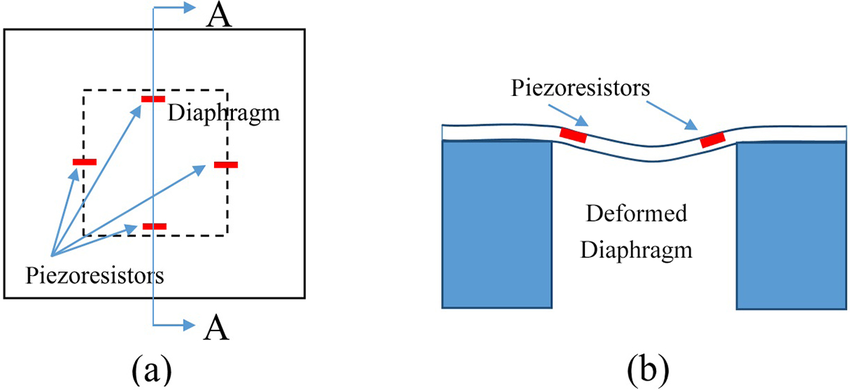
\includegraphics[width=10cm]{assets/figures/4_2_4_Pression_Keller_series26W.PNG}
    \caption{Capteur de pression de Keller, series 26 W (Source : Kubba 2016)}
    \label{fig:Pression_Keller_series26W}
\end{figure}

Ce capteur est utilisé pour mesurer des niveaux d'eau, indirectement en mesurant la pression due à la profondeur d'immersion. C'est la différence de pression avec la pression hors de l'eau qui est mesurée. Pour amener la pression atmosphérique au niveau de la membrane, un tuyau remonte en surface en passant dans le c‚ble (tube de ventilation).

\begin{figure}[h!]
    \centering
    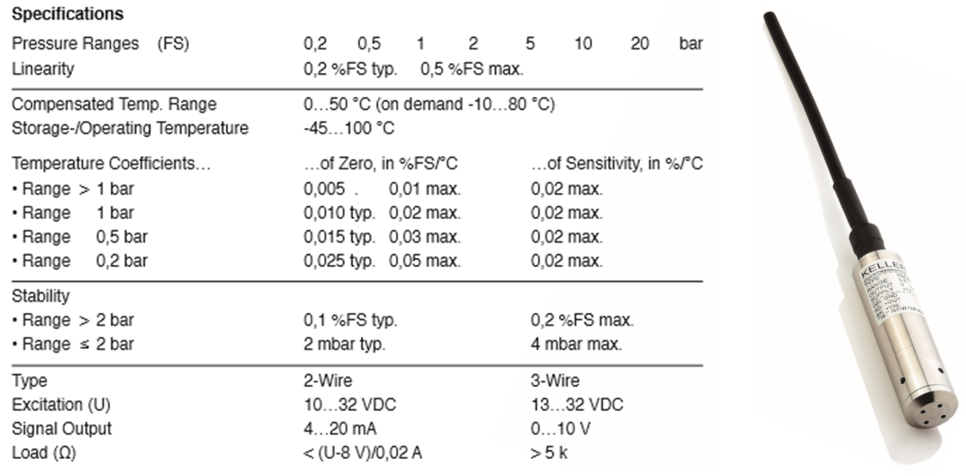
\includegraphics[width=15cm]{assets/figures/4_2_4_Pression_Keller_series26W_caracteristiques.PNG}
    \caption{Caractéristiques du capteur de pression de Keller, series 26 W}
    \label{fig:Pression_Keller_series26W_caracteristiques}
\end{figure}

\subsection{Jauges de déformation}
Dans une jauge, une déformation provoque une variation de la résistance. Cette variation de résistance répond à l'équation : \\
$\Delta R = k \ Delta L $
Avec :
$\Delta R$ : variation de résistance [$\Omega$]
$\Delta L$ : déformation [m]
k : coefficient ou facteur de jauge [$\Omega/m$]

\begin{figure}[h!]
    \centering
    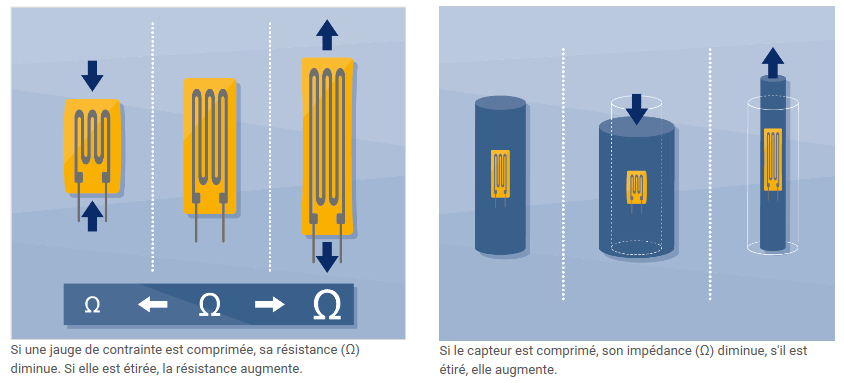
\includegraphics[width=15cm]{assets/figures/4_2_5_Jauges_de_deformation.png}
    \caption{Jauges de déformation (source HBM)}
    \label{fig:Jauges_de_deformation}
\end{figure}

Les jauges sont montées sur un corps d'épreuve. Les contraintes mécaniques entraînent une déformation. C'est cette déformation qui est mesurée par la jauge. Elle permet de retrouver la contrainte connaissant la rigidité du corps d'épreuve.


\subsection{Force (HBM RSCC)}

Les forces sont mesurées par la déformation d'un corps d'épreuve.
Pour ce capteur de force, des jauges de contraintes sont montées selon un pont de Wheastone sur les zones avec des contraintes mécaniques importantes et avec des paires où les contraintes mécaniques sont opposées (jauges 1-4 et 2-3).

\begin{figure}[h!]
    \centering
    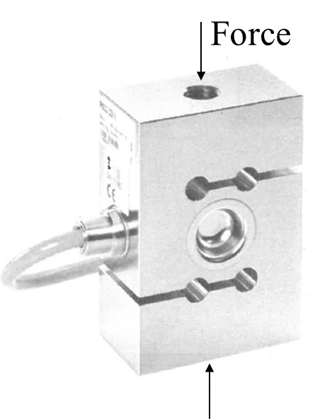
\includegraphics[width=7cm]{assets/figures/4_2_6_Force_HBM_RSCC.PNG}
    \caption{Capteur de Force HBM RSCC (source HBM)}
    \label{fig:Force_HBM_RSCC}
\end{figure}

\begin{figure}[h!]
    \centering
    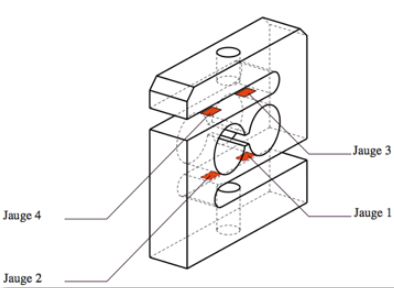
\includegraphics[width=7cm]{assets/figures/4_2_6_Force_HBM_RSCC_detail.PNG}
    \caption{Capteur de Force HBM RSCC: détails}
    \label{fig:Force_HBM_RSCC_detail}
\end{figure}

Le pont de Wheastone est composé de 4 résistances. Ces résistances sont remplacées par des jauges, avec une, deux ou quatre jauges, respectivement pour un quart de pont, demi-pont ou pont complet.
\begin{figure}[h!]
    \centering
    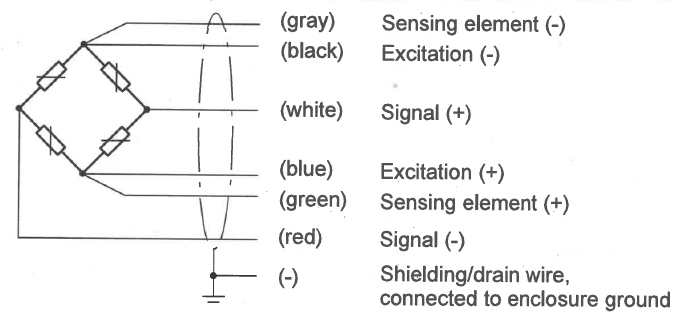
\includegraphics[width=7cm]{assets/figures/4_2_6_Force_HBM_RSCC_connexions.PNG}
    \caption{Capteur de Force HBM RSCC: connexions}
    \label{fig:Force_HBM_RSCC_connexions}
\end{figure}

\subsection{Couple (Omega TQ513)}
L'Omega TQ513 est un capteur de couple, basé sur des jauges de contraintes, placées sur une zone déformable (corps d'épreuve). Les jauges étant sur la partie tournante, un dispositif permet d'assurer le contact électrique glissant (slip rings).

\begin{figure}[h!]
    \centering
    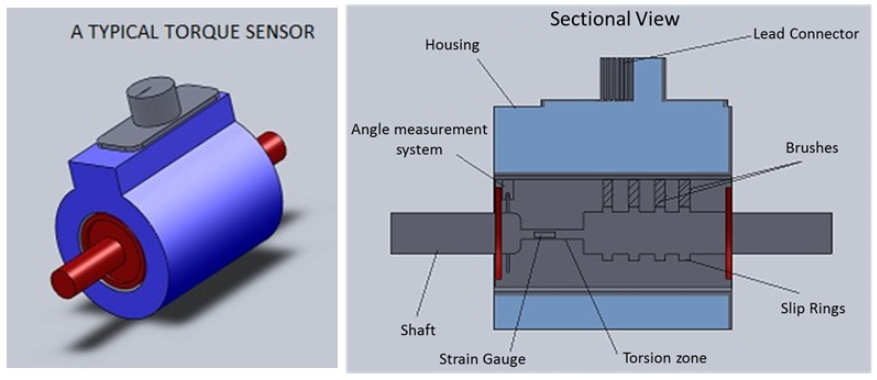
\includegraphics[width=7cm]{assets/figures/4_2_7_Couple_Omega_TQ513.PNG}
    \caption{Capteur de couple: Omega TQ513}
    \label{fig:Couple_Omega_TQ513}
\end{figure}

La déformation est liée aux propriétés mécaniques de la zone de torsion. Les jauges sont placées dans les axes de déformation maximale. Pour un pont complet, il y a une paire de jauge en compression et une paire en extension.


\begin{figure}[h!]
    \centering
    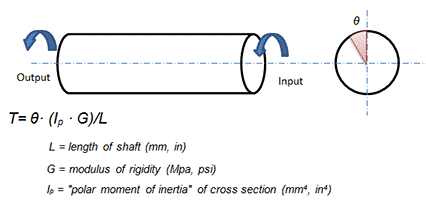
\includegraphics[width=7cm]{assets/figures/4_2_7_Couple_Omega_TQ513_principe.PNG}
    \caption{Principe du capteur de couple (Source : https://cecas.clemson.edu)}
    \label{fig:Couple_Omega_TQ513_principe}
\end{figure}

\subsection{Position linéaire (LT1300)}
Les capteurs LT1300 est un capteur de position linéaire, avec une gamme de 25 à 200mm.


\begin{figure}[h!]
    \centering
    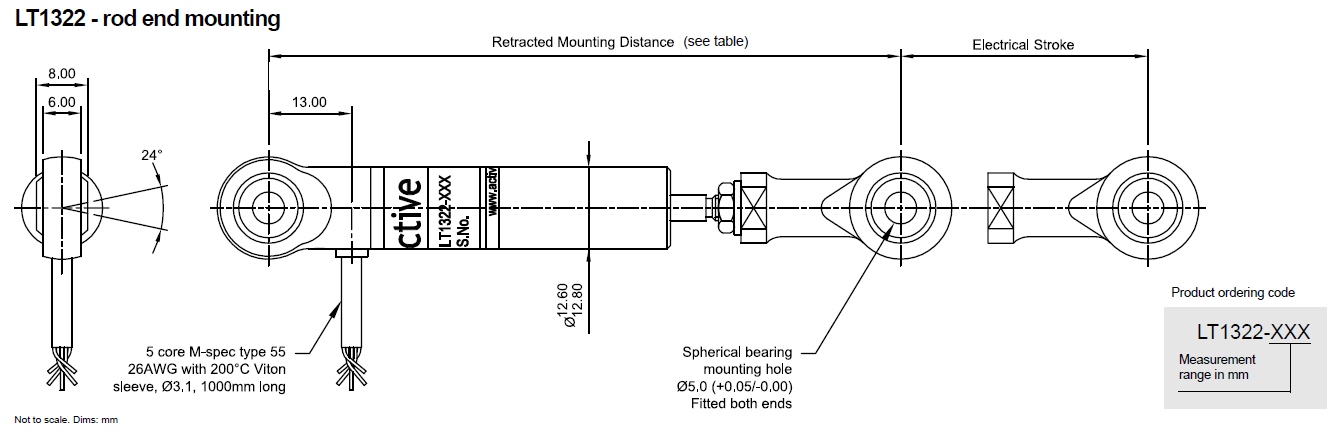
\includegraphics[width=7cm]{assets/figures/4_2_8_Position_lineaire_LT1300.PNG}
    \caption{Capteur de position linéaire LT1300}
    \label{fig:Position_lineaire_LT1300}
\end{figure}

Il fonctionne sur le principe du LVDT. C'est un principe inductif, utilisant un noyau ferromagnétique se déplaçant dans un transformateur pour modifier les couplages. Il utilise deux secondaires afin d'obtenir une réponse symétrique.

\begin{figure}[h!]
    \centering
    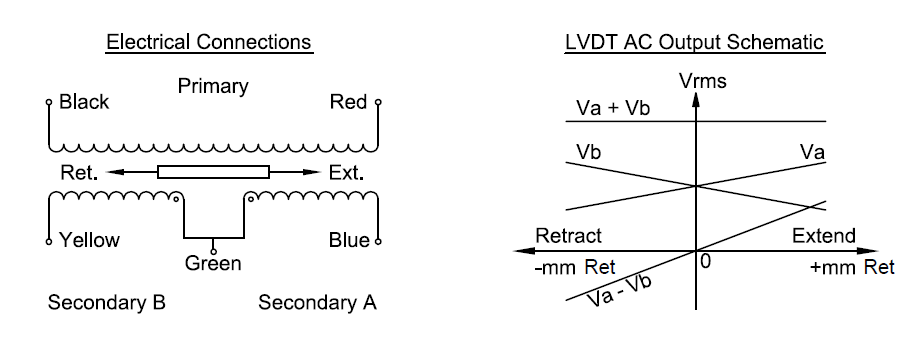
\includegraphics[width=7cm]{assets/figures/4_2_8_Position_lineaire_LT1300_detail.PNG}
    \caption{Capteur de position linéaire LT1300: principe}
    \label{fig:Position_lineaire_LT1300_detail}
\end{figure}

Un conditionneur de signal est nécessaire pour l'excitation du LVDT et pour effectuer la mesure. À noter que la réponse des LVDT n'est pas très linéaire, ce qui nécessite souvent une linéarisation.

\begin{figure}[h!]
    \centering
    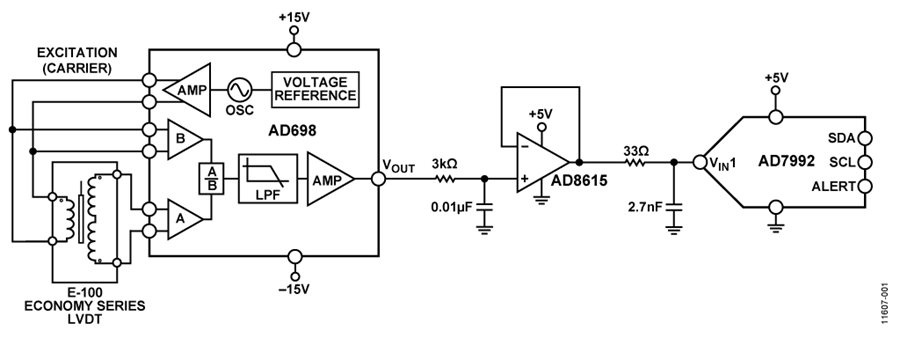
\includegraphics[width=7cm]{assets/figures/4_2_8_Position_lineaire_LT1300_conditionneur.PNG}
    \caption{Capteur de position linéaire LT1300: conditionneur}
    \label{fig:Position_lineaire_LT1300_conditionneur}
\end{figure}

\subsection{Position angulaire (Baumer GM400)}
Le Baumer GM400 est un codeur absolu. Il utilise un principe optique. Un disque codé avec des trous, tournant avec l'axe, permet de mesurer la position angulaire grâce à une source lumineuse est des photodétecteurs.

\begin{figure}[h!]
    \centering
    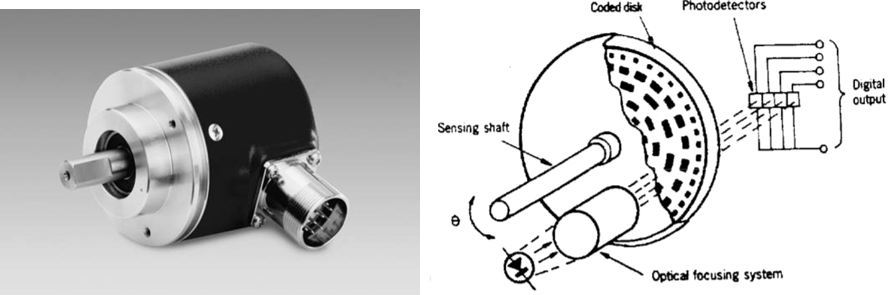
\includegraphics[width=7cm]{assets/figures/4_2_9_Position_angulaire_Baumer_GM400.PNG}
    \caption{Position angulaire Baumer GM400 (Sources : Baumer et Guy Gauthier)}
    \label{fig:Position_angulaire_Baumer_GM400}
\end{figure}

Pour certains codeurs optiques, le code binaire Gray est utilisé. Ce code offre l'avantage de ne modifier qu'un seul bit à la fois quand un nombre est augmenté d'une unité, contrairement au codage binaire naturel. Cela permet d'éviter des états transitoires lors des transitions.


\begin{figure}[h!]
    \centering
    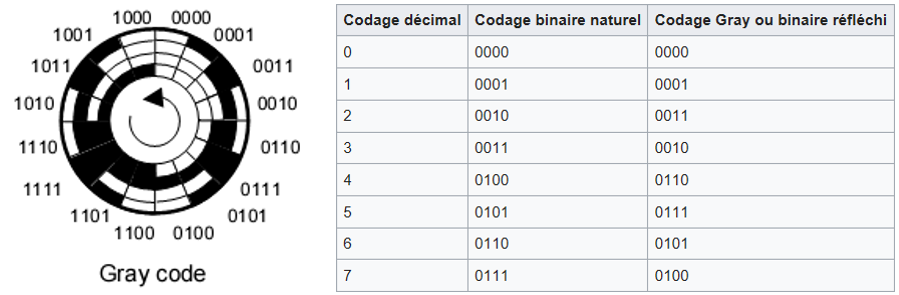
\includegraphics[width=7cm]{assets/figures/4_2_9_Position_angulaire_Baumer_GM400_codage.PNG}
    \caption{Position angulaire Baumer GM400: codage}
    \label{fig:Position_angulaire_Baumer_GM400_codage}
\end{figure}


Le transcodage binaire Gray/naturel est évidemment possible avec des algorithmes simples.

À noter que pour un capteur incrémental, deux signaux sont nécessaires pour connaître le sens de rotation. L'idée est d'utiliser deux signaux carrés déphasés de $90 \degree$.


\begin{figure}[h!]
    \centering
    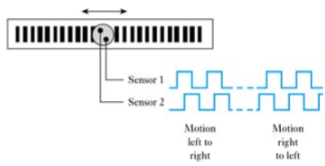
\includegraphics[width=7cm]{assets/figures/4_2_9_Position_angulaire_Baumer_GM400_fonctionnement.PNG}
    \caption{Position angulaire Baumer GM400: fonctionnement}
    \label{fig:Position_angulaire_Baumer_GM400_fonctionnement}
\end{figure}

\subsection{Vitesse (Philips KMI15/1)}
Le capteur de vitesse Philips KMI15/1 utilise un principe magnétique, avec une roue dentée ferromagnétique déformant le champ magnétique d'un aimant permanent.



\begin{figure}[h!]
    \centering
    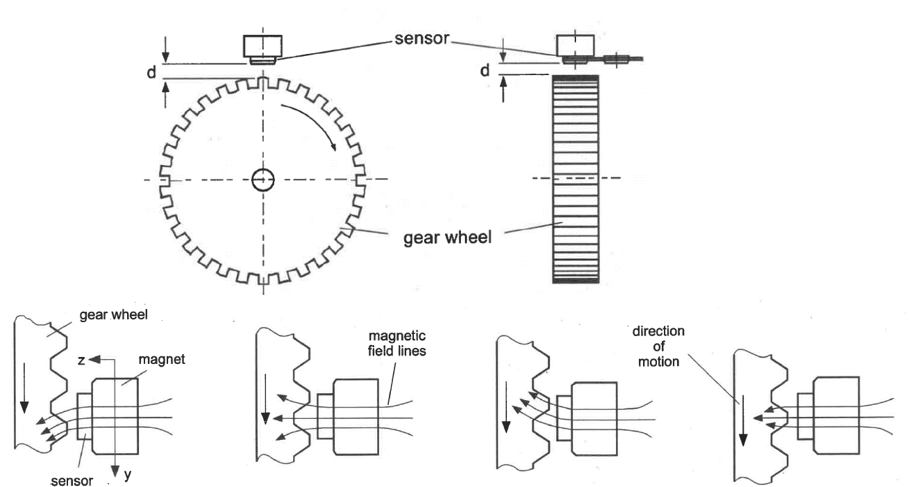
\includegraphics[width=7cm]{assets/figures/4_2_10_Vitesse_Philips_KMI15_1.PNG}
    \caption{Capteur de vitesse: Philips KMI15/1}
    \label{fig:Vitesse_Philips_KMI15_1}
\end{figure}

Le capteur KMI15/1 comprend l'aimant permanent et un capteur magnétorésitif (dont la résistance varie avec la magnétisation). La sortie du capteur est numérique de type tout ou rien (TOR).


\begin{figure}[h!]
    \centering
    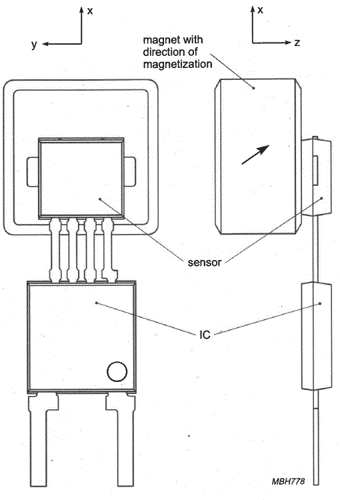
\includegraphics[width=7cm]{assets/figures/4_2_10_Vitesse_Philips_KMI15_1_detail.PNG}
    \caption{Détail du capteur de vitesse Philips KMI15/1}
    \label{fig:Vitesse_Philips_KMI15_1_detail}
\end{figure}

À noter encore que la mesure de vitesse avec une roue dentée est aussi possible en utilisant des capteurs de technologie inductive ou optique.


\subsection{Capteur de vibration (Colibrys VS1000)}

Le capteur de vibration Colibrys VS1000 est base sur une masse suspendue. Un principe capacitif permet de mesurer la position de la masse ou de créer des forces (pour le self-test)
Ce capteur dispose d'une sortie analogique radiométrique différentielle. Il dispose aussi d'une entrée pour lancer le self-test et d'un signal d'erreur en sortie. À noter encore la présence d'une mesure de température, souvent présente dans les capteurs intelligents.



\begin{figure}[h!]
    \centering
    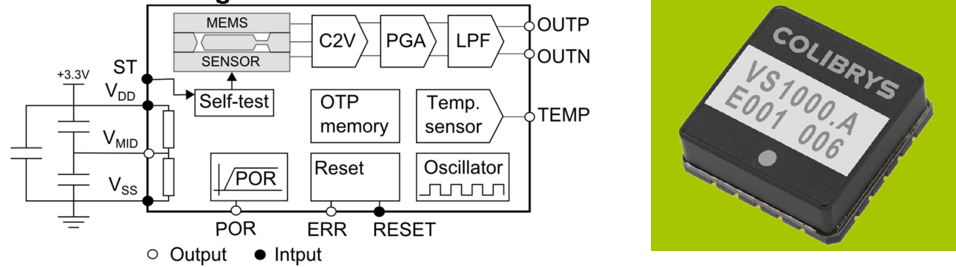
\includegraphics[width=7cm]{assets/figures/4_2_11_Capteur_de_vibration_Colibrys_VS1000.PNG}
    \caption{Capteur de vibration: Colibrys VS1000}
    \label{fig:Capteur_de_vibration_Colibrys_VS1000}
\end{figure}

\subsection{Capteur de proximité (Baumer CFDK 30N3600)}

Le capteur Baumer CFDK 30N3600 est un capteur de proximité capacitif. Il permet de détecter sans contact des objets métalliques et non métalliques à faible distance. Il permet aussi de détecter des niveaux de liquide à travers un réservoir. Un potentiomètre permet de régler la sensibilité du détecteur.

Ces capteurs de proximité disposent d'une sortie tout ou rien (TOR).

\subsection{Capteur chimique (Membrapor  CO/C-200)}

Les capteurs Membrapor  CO/C-200 sont des capteurs électrochimiques permettant la mesure de la concentration de monoxyde de carbone (CO). Pour ce type de capteurs, les dérives sont importantes, en particulier la dérive thermique, comme le montrent les graphiques ci-dessous.

\begin{figure}[h!]
    \centering
    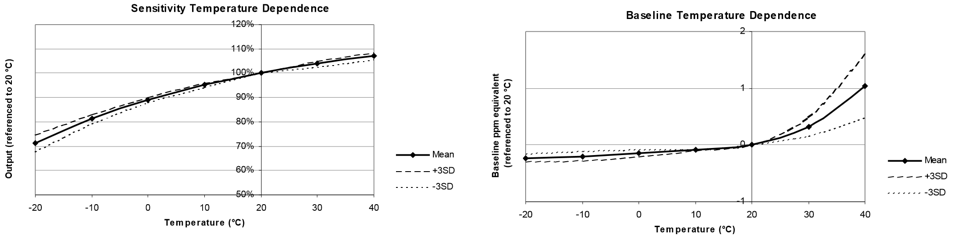
\includegraphics[width=7cm]{assets/figures/4_2_13_Capteur_chimique_Membrapor_CO_C_200.PNG}
    \caption{Capteur chimique: Membrapor  CO/C-200}
    \label{fig:Capteur_chimique_Membrapor_CO_C_200}
\end{figure}

À noter encore des grandeurs d'influence (cross-sensitivity) provenant d'autres gaz.

\begin{figure}[h!]
    \centering
    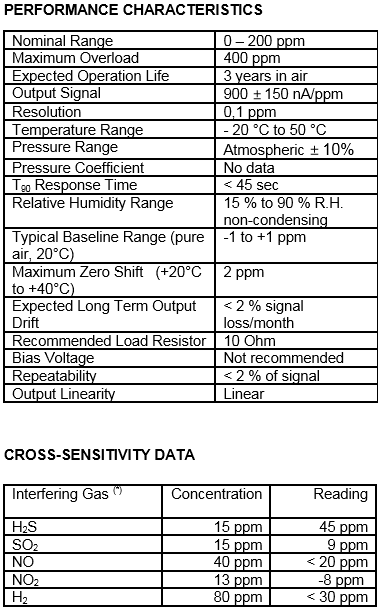
\includegraphics[width=7cm]{assets/figures/4_2_13_Capteur_chimique_Membrapor_CO_C_200_performance.PNG}
    \caption{Capteur chimique Membrapor  CO/C-200: performances}
    \label{fig:Capteur_chimique_Membrapor_CO_C_200_performance}
\end{figure}

\subsection{Capteur optique (Hamamatsu S-4251)}

Le capteur optique Hamamatsu S-4251 est constitué d'un driver pour une led exerne, une photodiode (c'est la raison du boîtier transparent) et une électronique de mesure utilisant le principe de la détection synchrone.

\begin{figure}[h!]
    \centering
    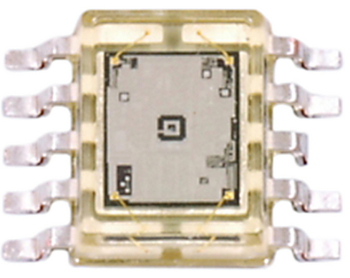
\includegraphics[width=7cm]{assets/figures/4_2_14_Capteur_optique_Hamamatsu_S_4251.PNG}
    \caption{Capteur optique:Hamamatsu S-4251}
    \label{fig:Capteur_optique_Hamamatsu_S_4251}
\end{figure}

Il y a souvent dans les capteurs des composantes de bruit à basses fréquences (bruit 1/f ou de la dérive). Il y a aussi souvent la présence de perturbations à basse fréquence. Par exemple des variations lentes de la lumière ambiante ou un scintillement à 50Hz. Le principe de la détection synchrone consiste à moduler le signal à mesurer pour se retrouver avec une fréquence plus élevée que ces bruits à basse fréquence.

\begin{figure}[h!]
    \centering
    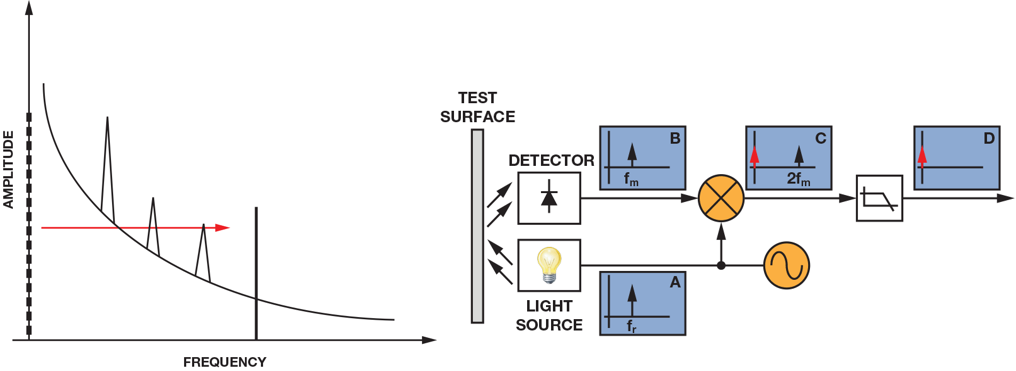
\includegraphics[width=7cm]{assets/figures/4_2_14_Capteur_optique_Hamamatsu_S_4251_conditionneur.PNG}
    \caption{Capteur optique Hamamatsu S-4251: exemple de conditionneur (source: Analog Devices)}
    \label{fig:Capteur_optique_Hamamatsu_S_4251_conditionneur}
\end{figure}

Dans ce capteur, le principe consiste à moduler la lumière vers 10kHz. Le signal reçu est alors démodulé en phase. Cela permet de s'affranchir de toutes les composantes de bruit à plus basse fréquence.

\subsection{Lectures conseillées}

\begin{itemize}
    \item " Les capteurs en instrumentation industrielle ", Georges Asch et Bernard Poussery, Dunod, 2017.
    \item " Acquisition de données, du capteur à l'ordinateur ", Gorge Asch, Dunod, 2011.
\end{itemize}

%\end{document}
